\section{Experiments}

\subsection{System setup}
A system with two articulated KUKA Lightweight-4 robots is built (Figure~\ref{fig:setup}): one robot is mounted with a motorized needle driver holding a curved needle while the second robot holds a mandrel with a stent graft. The mandrel, shown in Fig 2, is a cylinder with grooves for fixing the stent and is characterized by the presence of slots to allow the sewing. The stereo system is consisted of two Logitech C930E cameras. Calibration of the stereo system is performed by using the OpenCV library. The camera frame is registered to the robot frame by hand-eye calibration. By knowing the relative position between the robot and the needle driver, and the transformation between the robot frame and the camera given by the hand-eye calibration, the needle driver pose in the camera frame can be computed. The needle is initially grip at the very end of the needle driver and we assume that only small displacement of the needle pose will occur during the sewing task. The needle driver tip position is hence used as a prior of the needle position.

\subsection{Learning}
For teaching robot the sewing task, we carry out four demonstrations. All demonstrations starts from the same position and sew the same slot on the mandrel. To control the quality of the stitches, across all demonstrations the needle pierces in at the same location and pierces out at the same location. At the beginning of each demonstration, the needle is placed at the same place and normal to the needle driver.

The demonstrations are segmented into three primitive movements, according to the needle drive open and close even. Figure~\ref{fig:segment} shows one segmentation results. Figure~\ref{fig:demo} shows the demonstrated needle driver trajectories in 3D.

\begin{figure}
\centering{
{\includegraphics[width=8cm]{./fig/seg_37.eps}}
\caption{{Segmentation result of human demonstration. The red, green and blue patches label the three segments of the motion}}
\label{fig:segment}
}\end{figure}

\begin{figure*}
\centering{
\subfloat[\scriptsize{Demonstrations of phase 1}] {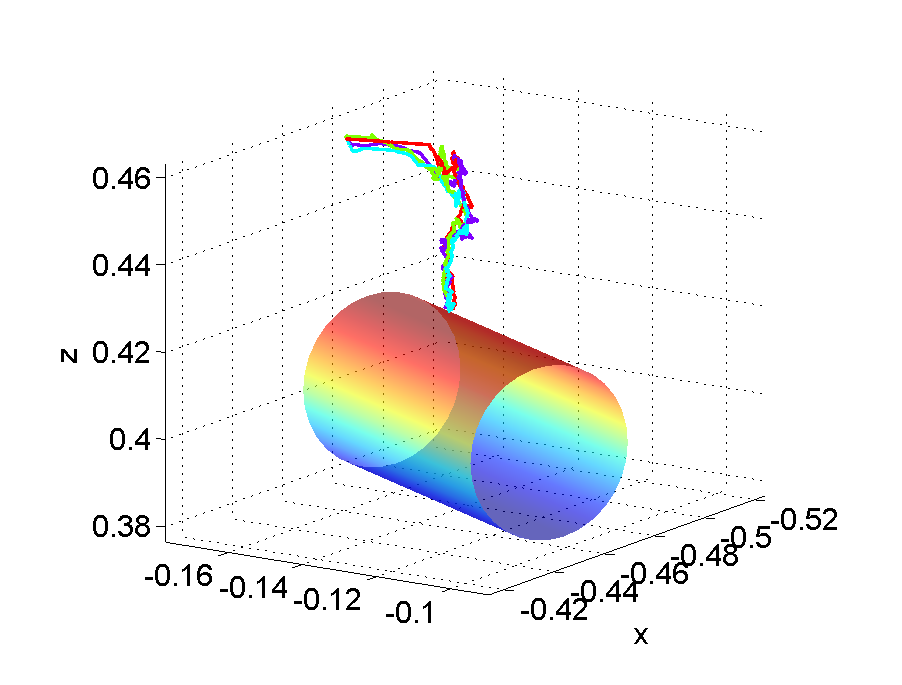
\includegraphics[width=4cm]{./fig/demo_1.eps}}
\subfloat[\scriptsize{Demonstrations of phase 2}]  {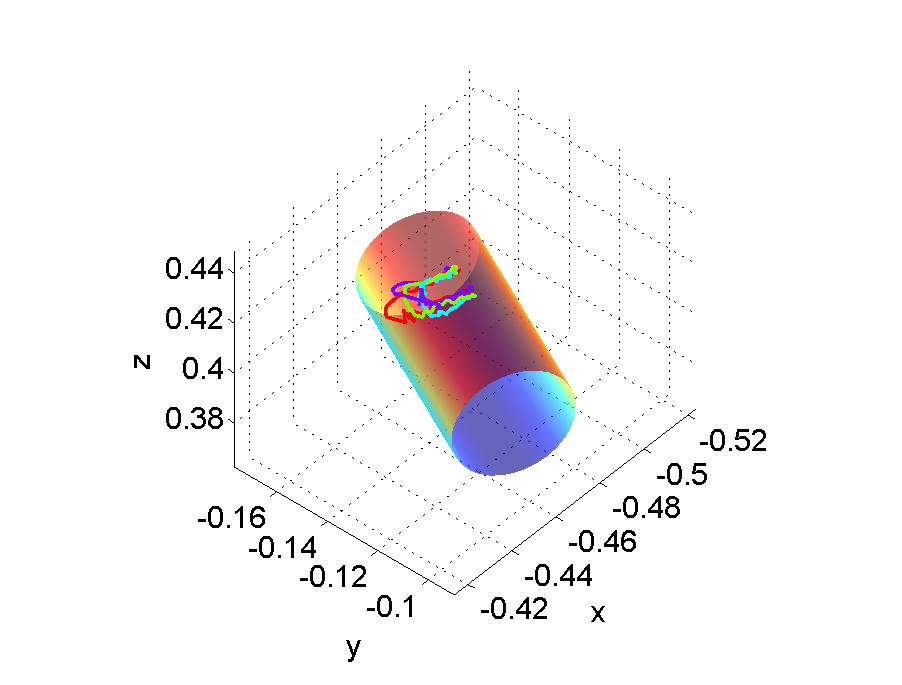
\includegraphics[width=4.5cm]{./fig/demo_2.eps}}
\subfloat[\scriptsize{Demonstrations of phase 3}]  {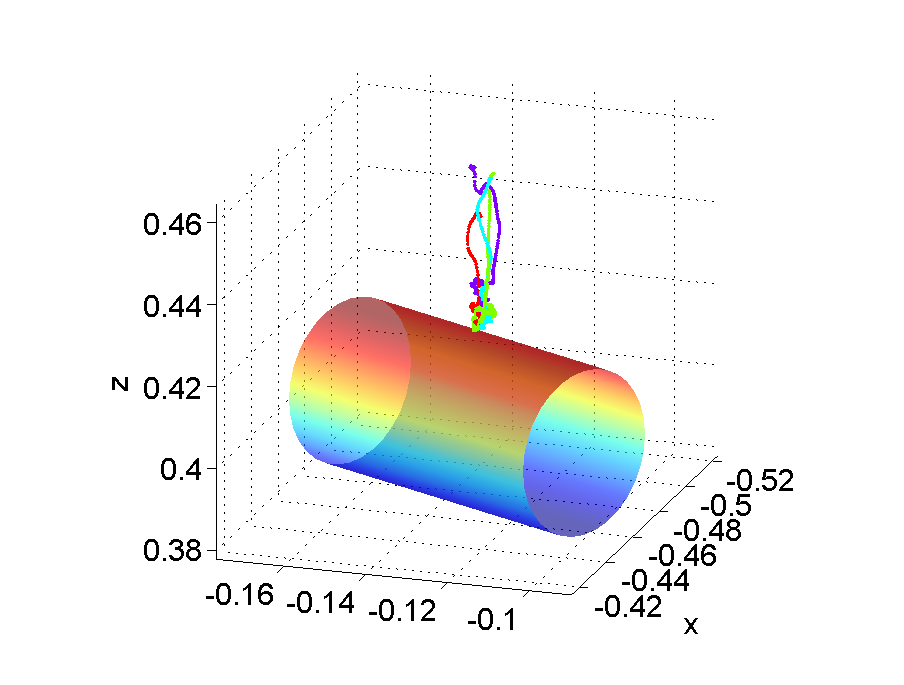
\includegraphics[width=4.5cm]{./fig/demo_3.eps}}
\subfloat[\scriptsize{Learnt trajectory of phase 1,2 and 3}]  {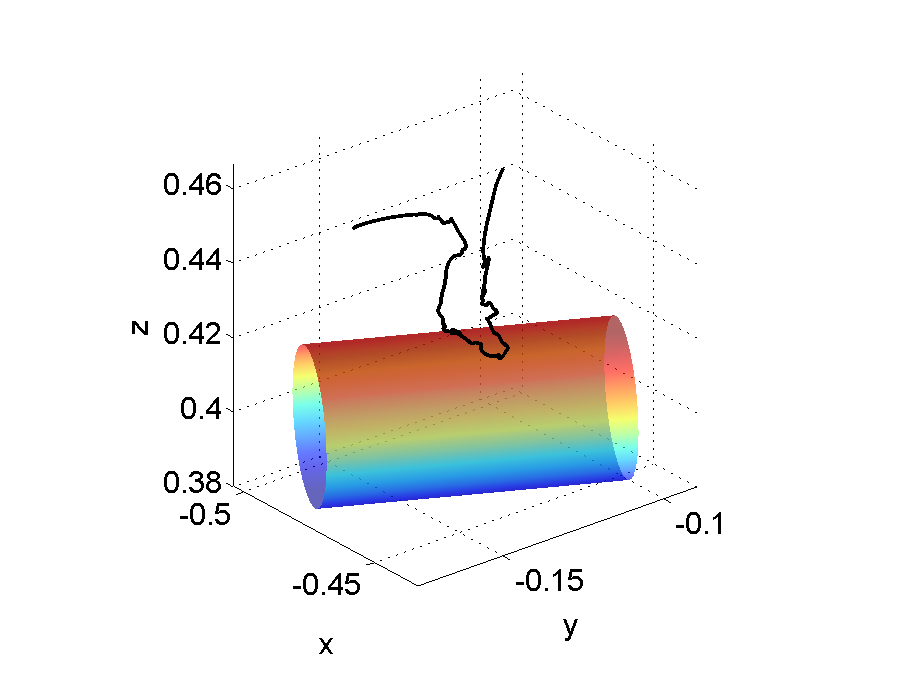
\includegraphics[width=4.5cm]{./fig/learn_123.eps}}
\caption{{Needle driver trajectories of human demonstrations and the learnt result. Each color represents one demonstration. The cylinder represents the mandrel}}
\label{fig:demo}
}\end{figure*}

GMM is used to learn model for each phase. Figure~\ref{fig:GMR} shows a 2D projection of the build model of each phase. It can be seen from the model that the three phases have different characteristics. Phase one has small variance from the beginning to the end, as all the movements start from the same point and pierce into the same location. The piercing movements are the same in order to produce similar stitches. Phase two has larger variance compare to phase one, as the needle is detached with the robot and the robot movement has less constraints. Phase three has small variance at the beginning, when the robot needs to pull out the needle from the same location, and has large variance once the needle is pulled out from the fabric. These show that the GMM can effectively capture the constraints at each phase and hence generate proper trajectories for the robot to complete the task.

\begin{figure*}
\centering{
\subfloat[\scriptsize{Phase 1}] {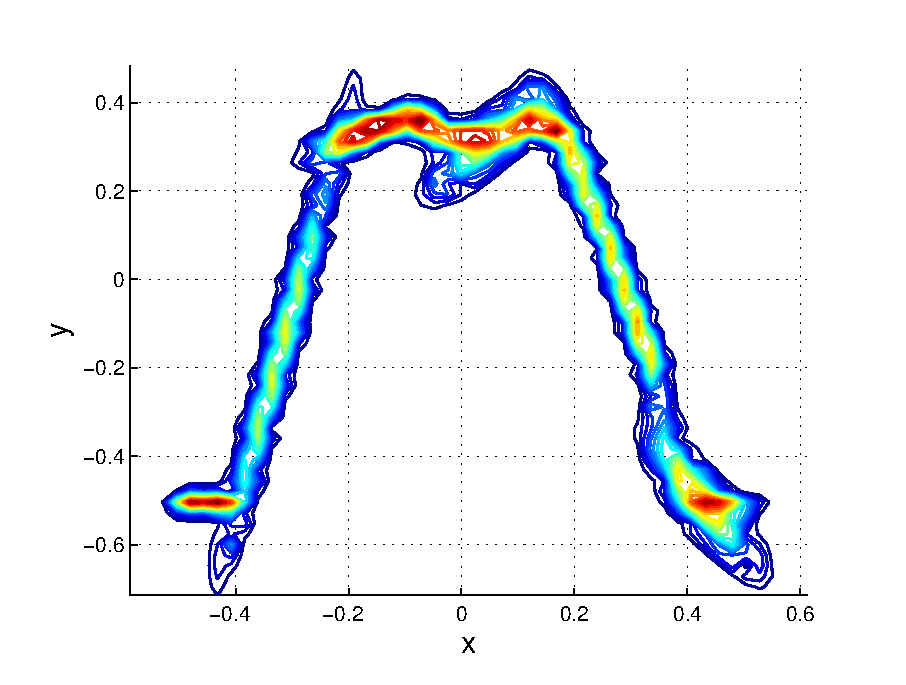
\includegraphics[width=6cm]{./fig/gmm_contour1_1-2.eps}}
\subfloat[\scriptsize{Phase 2}]  {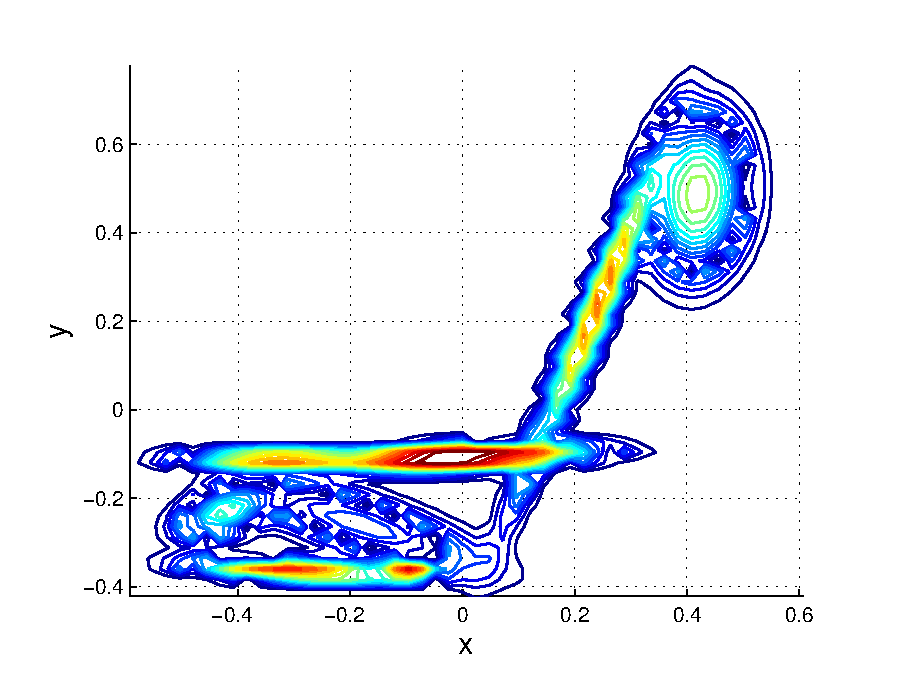
\includegraphics[width=6cm]{./fig/gmm_contour2_1-2.eps}}
\subfloat[\scriptsize{Phase 3}]  {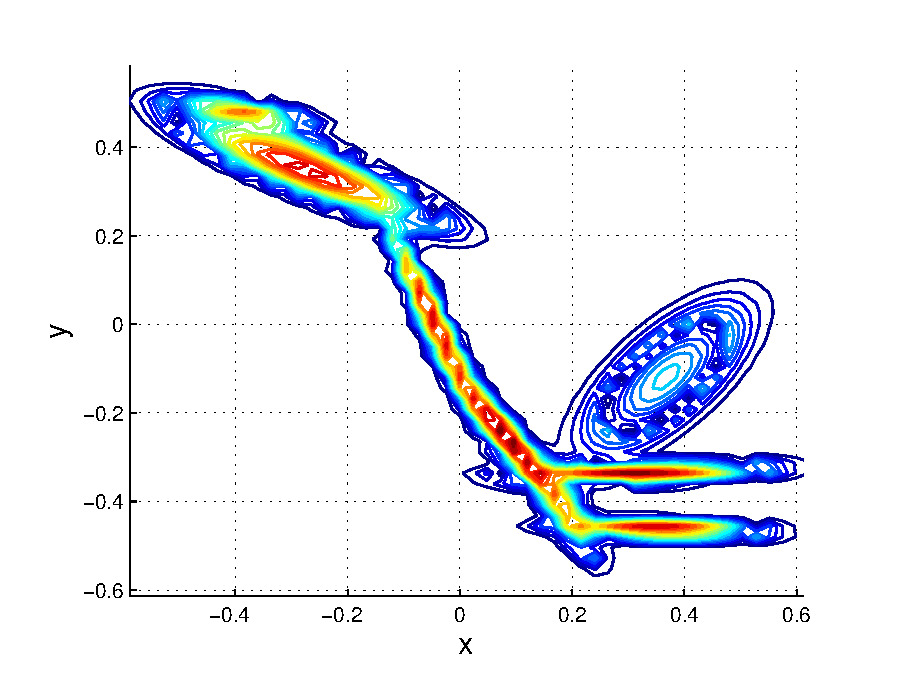
\includegraphics[width=6cm]{./fig/gmm_contour3_1-2.eps}}
\caption{{2D representation of the learnt models of different phases.}}
\label{fig:GMR}
}\end{figure*}

\subsection{Task execution}
Before starting replay the learned trajectory, a needle pose detection is performed using the stereo cameras and the transformation between the new needle pose and the optimal needle pose is calculated. Then a new needle driver trajectory is generated according to the transformation. If the needle pose is different with respect to the one presented during the demonstration, then the robot needs to adapt to a new pose in order to pierce the fabric in the same way it did during the demonstration.

In order to test our system to cope with variations on the needle pose, different needle poses are defined with respect to the one used during the demonstration, i.e. the optimal needle pose. A set of seven poses are defined where the variations ranges between 10mm translation along the grasper, and $±20°$ rotation respectively around the point being grasped. During the experiment, the system successfully coped with the needle pose variations six times and failed once, resulting in a $86\%$ of successful rate. The error in the piercing positioning into the fabric was less than $2$mm. The only failure occurred was caused by the joint limits of the robot, which were reached during the experiment involving a rotation of $-20°$ the needle. For the purpose of effective using joint range, a weighted Jacobian matrix is used with punishment on the most saturated joints. Figure~\ref{fig:firstExperiment} shows the results of the experiment for five different poses included the optimal needle pose.

\begin{figure*}
\centering{
{\includegraphics[width=12.0cm]{./fig/collageResults2.png}}
\caption{Qualitative results of the task execution are shown for five different initial needle positions. Detection of the needle in the images is reported in the first row, while the robot adaptation during the task execution is shown in the second and third row. The end of the task is in the last row.}
\label{fig:firstExperiment}
}\end{figure*}

Needle regripping is another important procedure for closing one stitching sequence. In order to sew continuously, the needle gripped by its tip point needs to be passed to another fixed needle driver. For this purpose, we demonstrate 3 trajectories for passing the needle between two needle drivers. At the start of the demonstration, the needle driver takes the needle and feeds it into another fixed needle driver. The fixed needle driver grip the middle point of the needle so that the moving needle driver can grip the needle back at its end point. Afterwards, the moving needle driver goes to the initial sewing position and the needle detection is performed for a new sewing cycle. Figure~\ref{fig:secondExperiment} shows the result of successful execution of the learned trajectory for the needle regripping task.

\begin{figure*}
\centering{
{\includegraphics[width=17cm]{./fig/secondExperiment.png}}
\caption{Sequence of images that shows the automated needle regripping between the two needle driver.}
\label{fig:secondExperiment}
}\end{figure*}

\subsection{Vision for needle pose estimation}
Extensive evaluation of the needle reconstruction algorithm is performed by estimating the 3D needle reconstruction error. This metric measures the distance between the reconstructed 3D shape and the ground truth shape of the needle. The ground truth is generated by segmenting manually the positions of the needle in each stereo image which are then used to find the ground truth 3D needle shape by triangulation. The 3D needle reconstruction error, i.e. $Dist(N_{gt}, N_{est})$, between the estimated needle, $N_{est}$, with respect to the ground truth shape, $N_{gt}$, is defined as:
\begin{eqnarray}
Dist(N_{gt}, N_{est}) = \frac{1}{w + f} \Biggl( \sum_{i=1}^{w} d_{min}(N_{gt}(i), N_{est}) \nonumber \\
+ \sum_{j=1}^{f} d_{min}(N_{est}(j), N_{gt}) \Biggr)
\end{eqnarray}
where $w$ and $f$ are the cardinality of the set of points of $N_{gt}$ and $N_{est}$, respectively, and $d_{min}(N_{gt}(i), N_{est})$ is the Euclidean distance between the $i^{th}$ point of $N_{gt}$ to the closest point on $N_{est}$. The distance $Dist$ is also presented in \cite{Walsum2005}. The mean and standard deviation of the 3D needle reconstruction error for the experiment involving seven different needle poses is $0.512 \pm 0.097$ millimetres. Thus, the needle reconstruction reaches sub-millimetres accuracy allowing a robust needle pose estimations which intrinsically depend on the needle reconstruction. 